% !TeX root = ../main.tex

\chapter{引言}

 \section{研究背景与意义}
% 
%C语言是一种面向过程的高级程序编程语言,在众多编程语言涌现并蓬勃发展的今天,仍具有较高的活跃度与旺盛的生命力。与其他语言对比,C语言的特点是明显的:作为一种高级语言,它可以直接操作低级处理器且无需任何运行环境,同时能够产生更少的机器码。
%

% 主题:基于区间的整数缺陷检测+基于精确值流图的程序理解与需求确认

在软件研发活动中,软件的验证与确认\cite{wagner2016functionally, wallace1989software}是十分重要的步骤。验证(verification)的目的是评估软件是否如软件定义般实现,而确认(validation)的目的则是评估软件是否符合预期的需求。在实际应用中,软件验证与确认经常会遇到困难。

对于前者而言,尽管软件需求是明确的,但在开发人员实际开发过程中经常会因为疏漏而不可避免的在软件中引入一些错误,导致软件缺陷的发生。其中,因整数计算问题直接或间接造成的缺陷不占少数,典型的如整型溢出、除零异常、内存泄露等。这些缺陷如得不到及时的发现与修复将会严重影响系统的稳定性与可靠性,在一些生命攸关的领域这些缺陷将会无限放大并造成难以估量的损失。

1995年,欧洲一研发时间超8年、耗资近80亿美元的阿丽亚娜5型运载火箭在发射40秒后发生爆炸,造成了巨大的经济损失。经事后排查,造成事故的原因是其导航系统试图将一个表示速度的浮点数转换为一个16位长的有符号整数。但在运行中该浮点数超过了整型变量的表示范围,导致转换失败。

时隔22年,人们在Linux内核的套接字模块中发现了一个因无符号减法造成运算溢出的问题,攻击者可以依照这个漏洞构造特殊的包套接字从而实现拒绝服务攻击和权限提升。通过这两个案例我们可以看出,整型缺陷问题一直存在且容易造成严重后果。如何在生产实践过程中及时、准确的找出整型计算造成的缺陷是十分重要的问题。

另一方面,软件确认也面临着较大困难\cite{wagner2013software}:要判断软件是否符合预期的需求,实际上是要判断软件实现与软件需求是否匹配。然而两者的描述方式是不同的,前者是具有复杂逻辑结构的代码,后者则是抽象的文字描述,相差较大。

面对这一问题,业界常用的方法是根据需求文档,逐条测试系统是否完成了相应需求\cite{ramler2006value}。但是该方法是不完备的:在软件分支条件复杂的情况下,人们往往不能穷举出程序所有可能的输入与执行路径,造成了软件确认的不完备。另一种常用方法是在确认时尝试理解代码,随后评估代码的逻辑是否与需求相对应。这种方案仍存在两个问题:(1)代码语义的精确理解是复杂的,过程中需要较多的人工介入\cite{ko2007information, murphy2006java, corbi1989program},难以很好的自动化;(2)软件需求本身的描述通常不够形式化,甚至大部分情况下不够具体。

为了解决上述整型缺陷检测以及软件需求确认中出现的问题,本文分别提出基于线性区间的整型缺陷检测方法与基于精确值流图的程序理解与函数摘要生成算法。

基于线性区间的整数缺陷检测方法拟解决如下问题:(1)对C语言整型变量进行抽象,借助静态分析对整型变量在程序运行时的取值范围做实时分析;(2)基于得到的分析结果,验证程序中是否存在整数缺陷,并生成缺陷检测报告。

基于精确值流图的程序理解与函数摘要生成算法拟解决如下问题:(1)自动抽取系统的语义,进而生成摘要信息供与用户进行需求比对;(2)根据生成的摘要内容进一步帮助用户细化需求。

 \section{研究现状}
 
 本节介绍整型缺陷分析所用关键技术的研究现状,包括抽象解释技术、数据流分析和符号化执行。同时介绍有关程序理解的研究现状。
 
 \subsection{抽象解释技术}
 
 论证程序正确性的方法最朴素的便是穷举程序所有可能的输入,并通过执行得到结果来判断其是否符合预期,如果运行结果符合预期,那么程序自然是正确的。然而,这种方法只是一种理论上可能的方法,在实际中,我们面对的程序输入的取值范围往往非常大,甚至无法穷举。以C语言的函数举例,若该函数有一个int型参数,由于int类型的表示范围是$ \left[  -2147483648, +2147483647 \right] $,那么单单一个int型参数就有$ 2^{32}  $种取值,当输入的参数是字符串类型时,更是有无穷多种可能。因此,使用朴素的穷举来进行程序分析,其时间与空间代价在实际中是不可接受的。
 
 当前常用的测试技术便是采用了上述思想,只不过测试技术所选择的输入是总输入空间的子集,通过边界条件分析等方法得到相对较少的输入空间。该方法的优点是大幅减少测试输入,但也带来了程序运行路径覆盖率低、需要人工参与测试输入样例的设计等问题。
 
 相较于测试技术,抽象解释技术采用了不同的思路。抽象解释是一种对程序语义进行可靠抽象(近似)的通用理论\cite{cousot1977abstract}。与此同时,该理论为程序分析的设计与构建提供了一个通用的框架\cite{cousot1979systematic}。具体地,它是将程序语义进行不同程度的抽象,并将这种抽象及在其上的操作称为抽象域。通过将具体域中的值与抽象域中的值进行映射,从而将具体域中数量庞大甚至无穷大的取值域转化为抽象域中的有穷的取值域。并将具体域上的操作对应到抽象域上的操作,通过在抽象域上计算程序的抽象不动点来表达程序的抽象语义。
 
 单纯通过构建在抽象域上的操作如迁移函数来进行建模有时并不能保证在程序的迭代分析中抽象域能快速到达不动点从而获得抽象语义。因此在抽象分析中提供了加宽算子(widening),通过上近似理论来减少程序分析中的迭代次数,从而加速程序分析。由于上近似理论的可靠性,所有基于上近似抽象得到的性质,在源程序中必定成立。
 
 抽象解释的核心问题是抽象域的设计,而如上所述,抽象解释是对程序语义的不同程度的抽象,这也就意味着抽象域并不唯一确定,针对特定问题可以设计使用特定抽象域以达到程序分析的效果。目前为止,已经出现了数十种面向不同性质的抽象域,其中,具有代表性的抽象域包括区间抽象域、八边形抽象域、多面体抽象域等数值抽象域\cite{张健2019程序分析研究进展}。另一方面,在开源领域出现了众多抽象域库,如APRON\cite{jeannet2009apron}、ELINA\cite{singh2017practical}、PPL\cite{bagnara2006parma}等。
 
 抽象解释并不是一个已经研究成熟的课题,当下抽象解释仍然面临着很多挑战,主要包括两方面的内容:提高分析精度与拓展性。在提高分析精度方面,主要要解决的问题是基于加宽算子(widening)的不动点迭代运算的精度损失问题以及所设计的抽象域本身的表达能力具有局限性的问题。而在提高可拓展性方面,主要面临的问题是如何有效降低分析过程中抽象状态表示与计算的时空开销。
 
 \subsection{数据流分析}
 
 通过抽象解释技术,我们能将具体域中的无穷状态问题转化为抽象域上的有穷的状态问题。而数据流分析则是在抽象解释的基础上,在控制流图上分析每个程序状态信息,从而得到每个静态程序点(语句)在运行时可能出现的状态。
 
 数据流分析是抽象解释的一个特例,经典的数据流分析理论\cite{aho1986compilers}使用有限高度的格$ <L,∩> $来表示所有可能的状态集合,其中$ L $是值集,是抽象域的别名;$ ∩ $是交汇运算,是将两个状态合并成一个状态的操作。由于在程序语句中存在循环控制语句,即存在循环结构,则数据流可能从不同分支流向同一节点。因此,为了得到不同分支的信息并保证算法的可终止性,需要定义交汇运算,将不同分支状态融合到同一节点上。
 
 数据流分析首先要确定数据流的方向,包括从Entry开始的正向分析和从Exit开始的逆向分析。数据流分析同时为每个程序语句构造一个单调的转移函数(又称变迁函数,transfer function),转移函数的输入是上一个程序点的状态信息以及程序语句,输出是程序语句执行后,下一个程序点应有的状态信息。
 
 用伪代码写成的数据流分析算法\cite{cooper2004iterative}如算法\ref{alg:数据流分析算法}所示:
 
 \begin{algorithm}[H]
 	\caption{数据流分析算法}
 	\label{alg:数据流分析算法}
 	\begin{algorithmic}[1]
 		
 		\Procedure{Recursion}{}
 		\State $ worklist = \emptyset $;
 		\For{$ i = 1$  to $ N $}
 		\State initialize the value at node $ i $;
 		\State add $ i $ to the $ worklist $;
 		\EndFor
 		\While{$ worklist \ne \emptyset $}
 		\State remove a node $ i $ from the $ worklist $;
 		\State recompute the data flow fact at $ i $;
 		\If{new data flow fact is not equal to the old one at $ i $}
 		\State add each successor/predecessor of $ i $ to $ worklist $ uniquely;
 		\EndIf
 		\EndWhile
 		\EndProcedure
 		
 	\end{algorithmic}
 \end{algorithm}
 
 相比于通用的抽象分析,经典的数据流分析在使用迭代计算框架来计算程序语句的不动点时,由于单调性和格的有限高度,保证了数据流分析的收敛性。因此相较于经典抽象分析技术,加宽算子对于数据流分析并不是必须的。
 
 \subsection{符号化执行}
 
 在上一小节的数据流分析中,我们讨论了数据流分析能够分析每个程序点上的状态信息,并能够保证算法的快速收敛。然而,算法的快速收敛的同时也混淆了不同路径上的信息,使得分析结果变得不明确。符号执行\cite{clarke1976system, king1976symbolic}提供了一种系统遍历程序路径空间的手段,除了保持状态信息外,还同时维护路径上的约束条件。符号化执行通过以符号值来代替实际值并在遇到分支条件节点时通过调用SMT求解器\cite{de2008z3}验证分支路径是否可达来实现路径的遍历。因此,求解器的能力是制约符号执行技术的一个重要因素。
 
 在多数情况下,静态分析方法的误报都是由于分析中不加判断的引入很多不可达路径,从而造成不合理判断。针对这种情况的误报,使用符号执行技术能够很有效的降低误报率。但是,符号执行也有它的弊端,那就是其对路径是敏感的,由此很容易产生路径爆炸问题,即,当一个程序具有n个条件判断语句结构时,理论上就有可能存在多达$ 2^n $条路径!尤其是当程序中存在无穷路径的循环结构时,符号执行算法甚至可能是无法终止的。在实际应用中,面对这种循环语句的情况通常采取的策略是仅展开有限次,配合其他静态分析方法对循环进行分析处理。
 
 目前,符号执行技术也面临着两方面的挑战,即提高可扩展性(scalability)与可行性(feasibility)。可扩展性指如何在有限的资源条件(内存、时间条件等因素)下提高符号执行的效率,从而更快完成分析。可行性指面对不同类型的分析目标如何应用符号执行技术,以及,如何权衡可靠性与准确性。在可扩展性方面,现有的研究主要围绕两种思路进行,其一是在具体目标下提供高效的搜索目标,其二是从约束输入范围着手,削减并合并路径从而达到减少程序路径空间的目的。
 
 \subsection{程序理解}
 
 
 %
 %该方法的核心是快速、自动化的从代码中抽取出程序语义,建立程序实现与需求之间的关系,帮助开发人员理解程序进行需求确认。程序理解\cite{boysen1979factors, sackman1968exploratory}领域以往的研究工作主要基于程序切片技术、程序标记技术以及执行可视化技术。
 %
 %程序切片技术\cite{binkley1996program}本质上是一种代码拆解技术。它通过剔除与指定变量不相关的代码语句,一定程度上减少了用户的代码阅读量。但是由于其并未能给出更上层的程序语义,用户仍需要阅读源码以获取知识。与之相反,程序标记技术\cite{sulir2017labeling}通过在源码上附加辅助信息的方式来帮助用户理解代码。现有工具可提供的辅助信息多种多样,但本质上用户仍要理解代码逻辑,并不能显著提升程序理解速度。执行可视化工具使用动态分析获取程序的执行信息并将之可视化,为了达到分析目的,工具将不同执行过程信息加以融合。其缺点是当程序逻辑复杂时,可视化的效果会变差,且需要为其配置程序运行环境,具有上手难度。 
 %
 %在条件分支众多、代码逻辑复杂的情况下,现有工具很难帮助用户理清程序输入输出变量之间的关系。文章\inlinecite{maalej2010can}指出,约25\%的代码维护工作流程是发现问题-修改-再验证的,同时,大量的开发者通过假设并验证程序的行为来理解软件\cite{maalej2014comprehension}。因此,若使用一种算法(工具)帮助开发者快速准确地抽取程序语义将会大大减少相关工作时间。
 %
 %本章中,作者提出了一种基于精确值流图(Value Flow Graph,简称VFG)的自动化程序静态分析算法,该算法通过使用指针分析得到内存模型,基于内存模型构造VFG,并进一步分析得到VFG上的程序语义。
 %
 %本方法是纯静态分析方法,不依赖于程序的具体执行路径,拥有较好的完备性。分析结果可用于开发人员进行程序理解和需求确认,也可以用于自动化的缺陷分析。
 
 
 目前有关程序理解的研究有很多,按照技术类别,可分为程序切片技术、程序标记技术、执行可视化技术。 
 程序切片技术于1979年首次被Weiser\cite{weiser1979program}提出,是一种可执行的后向静态分析。所谓可执行,是指切片后的结果仍是可编译可执行的,后向是指其结果包含切片准则所依赖的所有程序语句,静态是指它只使用程序的静态分析结果,即所有可能的执行都被考虑在内。该算法使用一个迭代的过程获取程序切片,首先在控制流图中找到每个节点的直接相关语句,然后每次迭代过程中都加入间接相关语句,当结果到达不动点时,程序终止。
 此方法的优点是得到的切片结果仍是可编译、可执行的独立代码段。然而正因保证了程序原有特性,其切片结果并没有显著减少,这意味着开发人员的代码阅读量并未因此降低多少。
 
 随后,由Korel和Laski\cite{korel1988dynamic}等人提出了动态切片技术,构造程序切片时采用了动态分析的技术,它能够根据程序的一次执行,获取程序在运行时的信息(尤其是指针、数组等),构造程序切片。由于动态切片的生成依赖于程序的执行,而程序的一次执行显然不能遍历所有执行路径,这就导致了切片结果不能包含可能相关的程序语句。优点是明显的:由于可以获取运行时的指针、数组等信息,其切片结果更加简单、准确。而缺点就是切片结果只针对特定输入,不具有兼容性。
 
 综合以上两种切片技术,Gupta\cite{gupta1997hybrid}等人提出了混合切片技术,它同时使用动态分析和静态分析来获取信息,并生成程序切片。然而由于程序切片本身的特性,它只能做到减少开发人员的代码阅读量,并不能为程序员提供代码之上的抽象信息,因此在使用程序切片时,仍需阅读代码以获得知识。 
 
 程序标记技术的提出的目的是为程序员提供更多信息,以方便理解代码。目前有大量的相关文章与工具:SE-Editor\cite{schugerl2009beyond}是一个Eclipse插件,通过使用超链接注释实现在代码内展示与代码相关的图表、视频等。Stacksplorer\cite{karrer2011stacksplorer}、RegViz\cite{beck2014regviz}和DepDigger\cite{beyer2010depdigger}等工具为源代码提供了视觉增强,如为函数提供图形化的调用信息、为正则表达式分组并标记组号以及根据变量的大小改变背景色等功能。还有一部分工具提供程序运行时信息,例如In-situ\cite{beck2013situ}会为函数创建包含运行性能信息的注释等。与本文工作较为类似的是\cite{haiduc2010supporting},它可以为函数提供摘要信息,然而这种摘要信息是以关键词的形式出现,仅阅读摘要并不能直接了解函数的行为。
 
 以上工具本质上都是为程序员提供辅助信息以帮助理解,但实际在应用过程中人们仍需要阅读源代码,理解速度并没有质的提升。 
 
 执行可视化工具如ExtraVis\cite{cornelissen2007understanding}和ExplorViz\cite{fittkau2013live}提供了另一种辅助理解的思路,这类工具在动态分析的基础上,基于多次执行,试图对程序的执行路径进行可视化。尽管这类工具创新性地提供了诸如Bundle View等视图,但由于其技术基础是动态分析,其兼容性不可避免地会减弱,不能够完整的表现程序在不同输入情况下的执行路径。同时,如果增加输入样例,则视图会变得更加复杂难以理解,违背了简化理解的初衷。另外,此类软件操作复杂,具有一定的学习成本,仍不适合快速理解代码。
 
 \section{研究内容与研究方案}
  
线性区间抽象域是当前常用的用于刻画程序中整型变量取值范围的一种抽象域,但是在实际应用中,因其存在着无法刻画整型变量的符号性、且因为抽象域本身表示能力问题带来的精度丢失,本文试图设计一个新的用于刻画整型变量的取值范围的抽象域,相比于独立的线性区间抽象域,它具有更强的表示能力、更高的分析精度。

另一方面,由于理解代码一直是软件开发乃至软件确认过程中耗时最大的工作部分。在面对逻辑复杂、软件条件分支众多的情况下,理解程序变成了十分具有挑战的工作。经调研,现有工具很难帮助用户理清程序输入输出变量之间的关系,因此本文试图提出一套算法(工具)来帮助开发者快速准确地抽取程序语义,加速程序的理解,从而提高人们的工作效率。

据此,本文的研究内容如下:  
 \begin{enumerate}
	\item \textbf{基于位敏感的区间代数的整型缺陷检测}:为了增强现有区间抽象域表示能力和精度上的不足,本文的研究工作之一是为C语言整型变量设计新的抽象表示。抽象域的设计应能体现整型变量的符号性,且在保证分析效率的情况下,具有较高的分析精度。另一方面,应设计抽象域上的变迁规则,从而实现程序分析并给出判定程序中是否存在整型缺陷的方法。
	
	\item \textbf{基于精确值流图的程序理解与需求确认}:为了提高开发维护人员对程序代码的理解效率,进一步加快程序确认流程,本文的另一个研究工作即是提出并设计一种程序理解方法,它可以自动化的抽取程序语义,并生成摘要,便于进一步的需求确认与缺陷分析。这种方法应能分析程序中的控制依赖与数据依赖,并准确生成不同路径条件下的变量关联信息。
	
	\item \textbf{工具研发}:本文的研究工作应具体实现为可用工具,并在一定的测试集上分析工具的可用性与工作效率。 	
 \end{enumerate}

\begin{figure}[H]
	\centering
	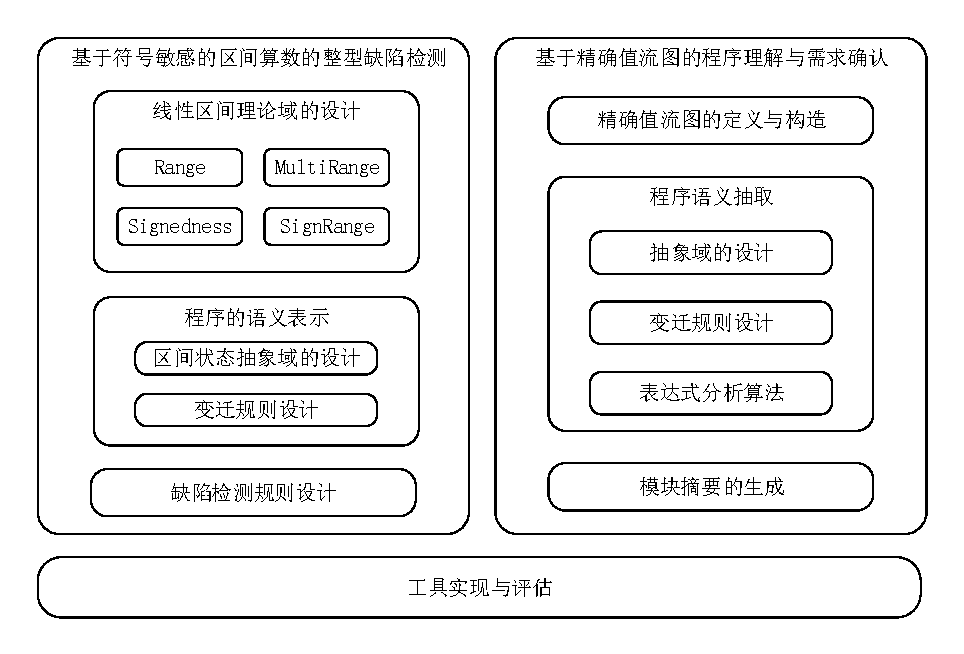
\includegraphics[width=6in]{YanJiuFangAn.pdf}
	\caption{研究方案}
	\label{fig:研究方案}
\end{figure}

  基于上述三点研究内容,本文提出如图\ref{fig:研究方案}所示的研究方案。
  
  \begin{enumerate}
  	\item 针对基于位敏感的区间代数的整型缺陷检测,本文进行如下三个方面的工作:其一是线性区间理论域的设计。为了增强现有区间抽象域表示能力和精度的不足,本文依次定义了线性区间Range、线性多区间MultiRange以及位敏感的线性多区间SignRange并设计了其计算规则。最后定义的SignRange能够较好的表示程序中整型变量的可能取值范围。其二,为了实现程序的语义表示,我们设计了区间状态抽象域RangeState来描述程序的每个状态,并通过定义变迁规则,模拟程序状态的变迁,从而实现程序的语义分析。最后,通过在RangeState上设计缺陷检测规则,实现程序的整型缺陷检测。
  	
  	\item 针对基于精确值流图的程序理解与需求确认,本文首先通过一个具体案例剖析使用基于值流图的程序理解方法为需求确认过程带来的好处,并以此展开,对该方法的具体内容做出了介绍。具体地,首先对精确值流图的定义与构造做出说明,基于精确值流图,设计了程序语义抽取方法。具体内容包括抽象域的设计、变迁规则的设计和表达式分析算法的设计。在上述的基础上,我们可以对程序整型变量在不同程序路径下的取值关系进行语义抽取。最后,利用得到的信息生成模块摘要。
  	
  	\item 最后,本文对上述两个研究方案中提出的方法进行编码实现,并设计相关实验,验证其正确性与实用性。
  \end{enumerate}
  
 
 \section{论文贡献}
 
 本文的贡献如下:
 \begin{enumerate}
 	\item 设计了表示能力更强的线性区间抽象域与变迁规则,使用它可以抽象表示程序在不同状态下整型变量的整数取值范围,进一步地,实现了针对C语言的整数缺陷检测方法;
 	
	\item 设计实现了一种基于内存模型的精准值流图分析构造方法,可处理动态内存空间、指针别名等传统数据流分析无法处理的语义关系,可区分数据流依赖、控制流依赖等依赖条件。同时,这一过程可自动化,并进一步可用于需求确认和缺陷分析,提升程序理解效率,提高代码质量;
	
	\item 基于上述两点,分别编码实现了相关工具并开展相关实验,证明了其正确性与实用性。
 \end{enumerate}
 
 \section{论文组织结构}
 
 本文的组织结构如下:
 
 第一章从软件验证与确认的角度介绍了整型缺陷分析与程序理解的相关背景知识与研究现状,并针对当前现状提出本文所研究内容与研究方案。
 
 第二章介绍了基于区间代数的整数缺陷检测方法,首先介绍了有关控制流自动机与可配置程序分析框架的基础知识,随后依次介绍扩展的整数(RangeInteger)、线性区间(Range)、线性多区间(MultiRange)和位敏感的线性多区间(SignRange)的理论域与计算规则的设计。我们以区间状态(RangeState)作为控制流自动机上状态节点的抽象表示,同时通过设计区间状态域上的变迁规则与整型缺陷检测规则,实现C语言上的整数缺陷检测。
 
 第三章介绍了基于精确值流图的程序理解与需求确认方法,首先通过一个机动车变速器控制逻辑的软件需求与实现的具体案例,介绍了程序理解对软件开发的重要性,并提出使用摘要来降低程序理解的难度。后续内容具体介绍了基于精确值流图的程序理解与需求确认方法的具体实现,包括抽象域、变迁规则的设计。在此基础上,介绍了变量关系分析方法、相关的程序理解方法与摘要的生成算法。
 
本文于第四章对上述问题的解决方法做了具体实现,并分别为两者设计了实验。通过实验验证了工具(算法)的有效性与实用性。随后,本文对实验中存在的误报、精度不足等问题做了具体分析并提出相关改进方案与技术展望。

第五章对本文所做工作进行了总结,并提出研究展望。
 
 
 
 
 
 
 
 
 
 
 
 
 
 
 
 
 
 
 
 
 
 
 
 
 
 
 
 
 
 
 
 
 